\chapter{Interactive Perception Library}
\label{chapter:Interactive Perception Library}


\section{Motivation and Goals}
Based on the increasing popularity of the interactive perception approach we created a common place that can unite other people' efforts towards better algorithms and systems that concern adding manipulation in the perception loop. Since we understand the world based on functionality and behavior, as a result, manipulation becomes an integral part of perception. In other words, purposeful manipulation depends on the robot's ability to curiously explore its unknown environment through interaction. 

It is worth emphasising and it has been shown in the \ref{chapter:Related Work} that interactive perception field has gained many more potential applications than the ones presented in this thesis. These areas include interactive perception methods for object segmentation, modeling, grasping, and even learning manipulation skills through interactive perception. Interestingly, these results are beginning to appear independently in the different relevant communities: perception, grasping, manipulation, and learning.

Having this in mind we created a common, modular tool - Interactive Perception Library \footnote{\url{http://github.com/Lolu28/interactive_perception}} that can address researchers' needs to investigate interactive perception area more deeply and it can enable easier access to existing resources and algorithms. The main goal of this library is to collect all the code from different laboratories being involved in the idea of interactive perception. We came up with a framework that enables to switch between different implementations of each step from the interactive perception pipeline at runtime. 


\section{Library}
\subsection{Steps}
Looking at various systems created by different robotics institutes REF it can be noticed that there is a similar idea lying behind them.  

After conducting research in existing implementations we noticed many similar steps that became crucial for our library, those being:

\begin{itemize}
\item Static Segmentation - to infer which parts of the scene are most likely being segmented incorrectly
\item Feature Extraction - to extract features that will be tracked
\item Push Point - to find the best point to interact with objects
\item Manipulation - to manipulate a robot in order to interact with objects in the scene
\item Tracker - to track previously extracted features during robot's movement
\item Trajectory Clustering - to cluster the trajectories of the features that have moved in the same manner
\item Full Reconstruction - to reconstruct a full model of the object. It takes the sparse representation - clustered features - and reconstructs a dense model of the object.
\end{itemize}




The library was created based on the abstract factory pattern and it is mainly using pluginlib \footnote{\url{http://ros.org/wiki/pluginlib}} from ROS. The main executable  shows a small user interface together with a visualization tool(visualizer package). The user interface shows possibility to call different steps and implementations of these steps by using a small GUI - dynamic reconfigure package \footnote{\url{http://www.ros.org/wiki/dynamic_reconfigure}}. The details are described in the next section.

\subsection{Architecture}

In order to describe the architecture it is needed to explain the idea of the pluginlib library that was heavily used in this project. Pluginlib is a C++ library that enables to load and unload other classes (plugins) dynamically without being explicitly linked   

Pluginlib is a C++ library for loading and unloading plugins from within a ROS package. Plugins are dynamically loadable classes that are loaded from a runtime library (i.e. shared object, dynamically linked library). With pluginlib, one does not have to explicitly link their application against the library containing the classes -- instead pluginlib can open a library containing exported classes at any point without the application having any prior awareness of the library or the header file containing the class definition. Plugins are useful for extending/modifying application behavior without needing the application source code. 

\begin{figure}[ht]
%\centering

{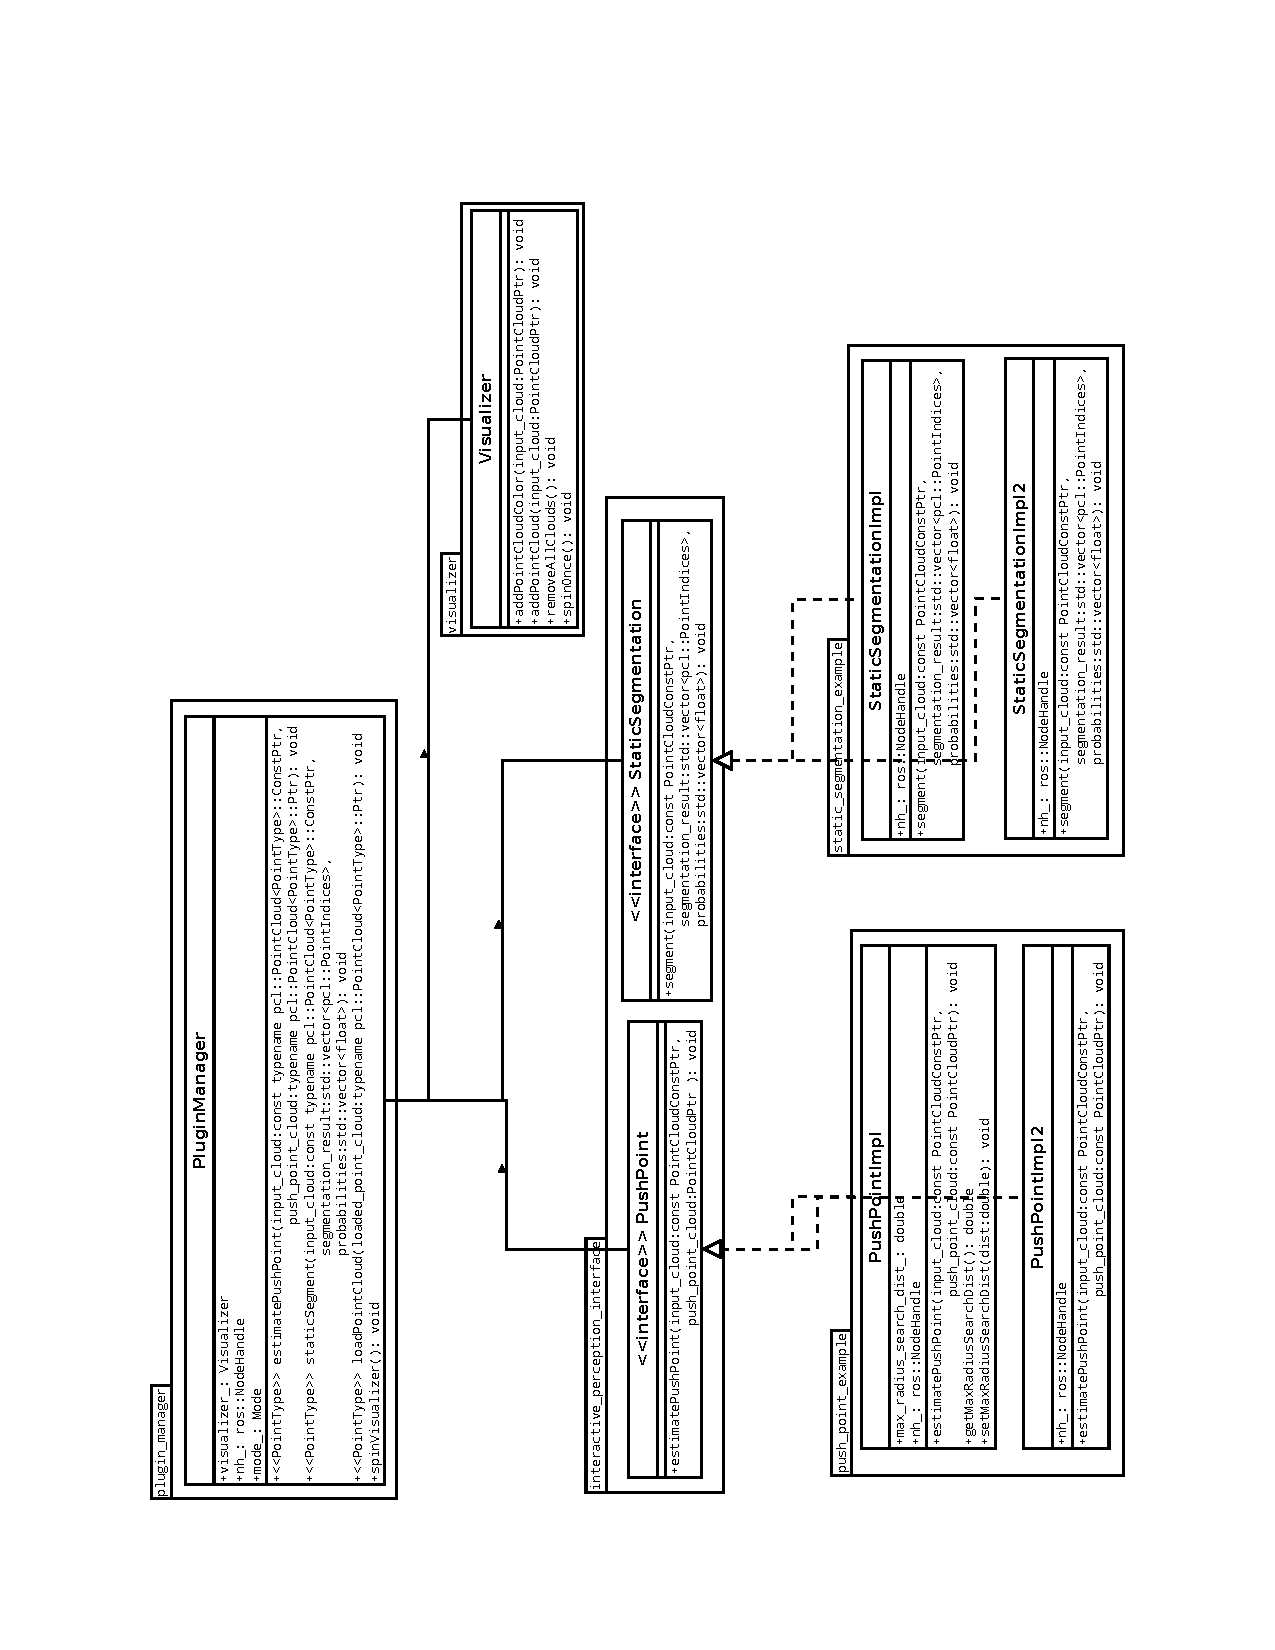
\includegraphics[width=1.1\columnwidth, angle=-90]{figures/uml2.pdf}}

\caption{Interactive Perception Library with running visualizer and a small Graphical User Interface to choose the step and its implementation.}
\label{fig:uml}
\end{figure}



\begin{figure}[ht]
%\centering

{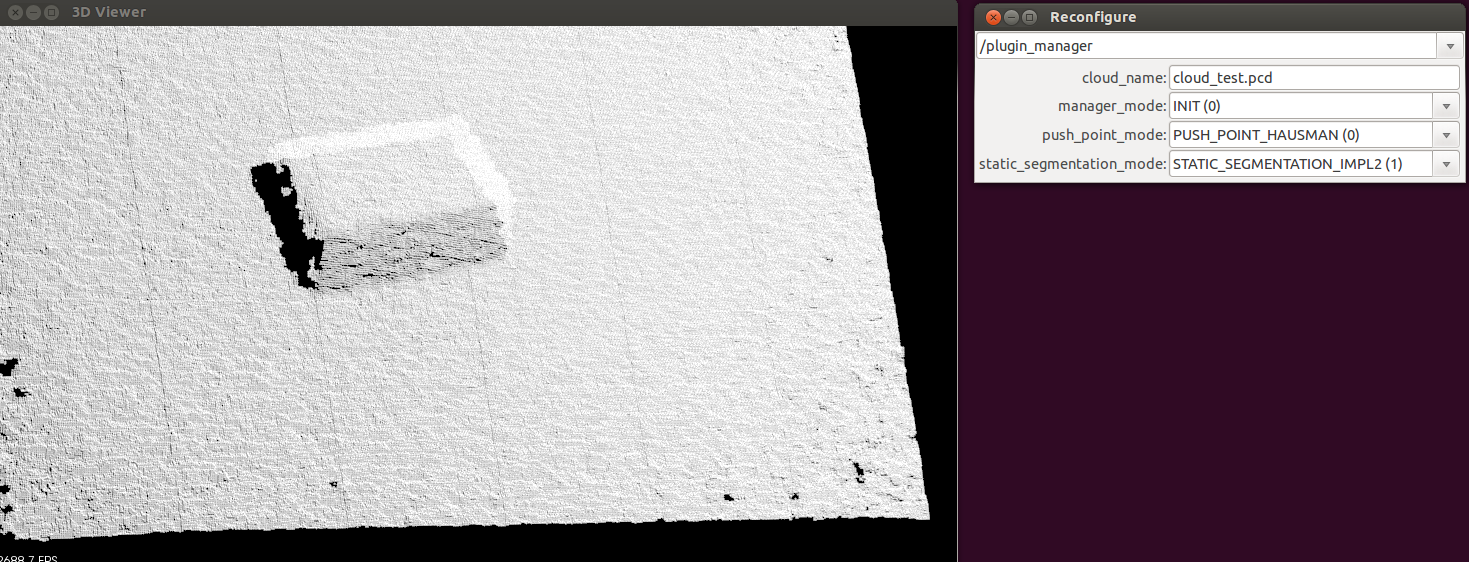
\includegraphics[width=1.1\columnwidth]{figures/ipl.png}}

\caption{Interactive Perception Library with running visualizer and a small Graphical User Interface to choose the step and its implementation.}
\label{fig:ipl}
\end{figure}

TODO		
 UML diagram
 screens from visualizer and dyn rec
 more about pluginlib and maybe abstract factory
